\subsubsection{Lecture 5 (20. Januar 2025)}

\section*{Gradient Descent}


Gradient descent er en metode for å finne minimum av en funksjon $f: \R^n \to \R$ ved å iterere:
\[
    x_{k+1} = x_k - \alpha_k \nabla f(x_k),
\]
hvor $\alpha_k$ er en skalar som kalles \emph{learning rate}.

\begin{remark}{Armijo condition}{}
    Armijo condition er en tilnærming for å velge $\alpha_k$ i gradient descent. Den sier at vi velger $\alpha_k$ slik at
    \[
        f(x_k - \alpha_k \nabla f(x_k)) \leq f(x_k) - c \alpha_k \norm{\nabla f(x_k)}^2,
    \]
    hvor $c \in (0, 1)$ er en konstant.
\end{remark}


\begin{algorithm}
    \caption{Backtracking gradient descent}
    \SetAlgoLined
    \KwIn{$f$, $\nabla f$, $x_0$, $\alpha_0$, $c \in (0, 1)$}
    $k \gets 0$\;
    \While{not converged}{
        $\alpha_k \gets \alpha_0$\;
        \While{$f(x_k - \alpha_k \nabla f(x_k)) > f(x_k) - c \alpha_k \norm{\nabla f(x_k)}^2$}{
            $\alpha_k \gets \beta \alpha_k$\;
        }
        $x_{k+1} \gets x_k - \alpha_k \nabla f(x_k)$\;
        $k \gets k + 1$\;
    }
\end{algorithm}


\begin{theorem}{}{}
    Assume that $f \in \mathcal{C}^2$, that $(x_k)_{k \in \N}$
    is generated by backtracking gradient descent with
    $x_0 \in \R^d$, $\hat{\alpha} > 0$,$c \in (0, 1)$, $\nabla f(x_k) \neq 0 \; \forall \; k$, and that
    $L_f(f(x_0))$ is bounded. Then, $\nabla f(x_k) \to 0$ as $\abs{x_{k+1} - x_k} \to 0$.
\end{theorem}

\begin{proof}{}{}
    \begin{enumerate}
        \item \textit{Boundedness of Iterates:} Since $L_f(f(x_0))$ is bounded and the backtracking gradient descent ensures $f(x_{k+1}) \leq f(x_k)$, the sequence $\{x_k\}$ remains within $L_f(f(x_0))$, hence bounded.
        \item \textit{Lipschitz Continuity of Gradient:} Given $f \in \mathcal{C}^2$ and $\{x_k\}$ is bounded, the gradient $\nabla f$ is Lipschitz continuous on $L_f(f(x_0))$. Thus, there exists $M > 0$ such that

              \[
                  \|\nabla f(x) - \nabla f(y)\| \leq M \|x - y\| \quad \forall x, y \in L_f(f(x_0)).
              \]

        \item \textit{Lower Bound on Step Sizes:} If $\|\nabla f(x_k)\| \geq \delta > 0$, the Armijo condition ensures a step size $\alpha_k \geq \alpha_{\min} > 0$ for some $\alpha_{\min}$, preventing $\alpha_k$ from shrinking to zero.
        \item \textit{Contradiction Argument:} Assume $\|\nabla f(x_k)\|$ does not converge to zero. Then, there exists $\delta > 0$ and an infinite subsequence where $\|\nabla f(x_k)\| \geq \delta$. Consequently, each such iteration decreases $f$ by at least $c \alpha_{\min} \delta^2$, leading to $f(x_k) \to -\infty$, contradicting the boundedness of $L_f(f(x_0))$.
    \end{enumerate}

    \textbf{Conclusion:} Therefore, $\|\nabla f(x_k)\| \to 0$. Since $\|x_{k+1} - x_k\| = \alpha_k \|\nabla f(x_k)\|$ and $\alpha_k$ is bounded below by a positive constant when $\|\nabla f(x_k)\|$ is not small, it follows that $\|x_{k+1} - x_k\| \to 0$ if and only if $\|\nabla f(x_k)\| \to 0$.

\end{proof}

\begin{remark}{}{}

    The result does not state that the sequence $\{x_k\}_{k \in \N}$ converges to a critical point.

    If all critical points of $f$ are isolated, then $\{x_k\}_{k \in \N}$ converges to a critical point.
\end{remark}

One can show: if the Hessian at all critical points is non-singular, then the sequence does not converge to a local minimum.
More generally, the theorem holds for search directions:

\[
    p_k = - B_k^{-1} \nabla f(x_k),
\]

where $B_k$ is a symmetric positive definite matrix.

\[
    \text{if } \exists C > 0 \text{ s.t. } \norm{B_k}_2 \leq C \text{ and } \norm{B_k^{-1}}_2 \leq C \text{ for all } k \in \N
\]

Choice of constant: $c_1 \approx 10^{-3,-4}$, $\rho \approx 10^{-1,-2}$.

\subsection*{Alternative methods for step length selection}

Armijo condition:
\[
    f(x_k - \alpha p_k) \leq f(x_k) - c \alpha \ip{\nabla f(x_k)}{p_k} \tag{(A)}
\]

if $(A)$ fails $\alpha$ is to large $\to$ decrease $\alpha$.

\begin{figure}[H]
    \centering
    \caption{Visualization of Armijo condition. The blue curve shows the actual function value, while the red dashed line shows the upper bound from Armijo condition. When $\alpha$ is too large, we reduce it until the function value falls below the Armijo bound.}
\end{figure}

\subsubsection*{Goldstein conditions}
Choose $0 < c_1 < c_2 < 1$.
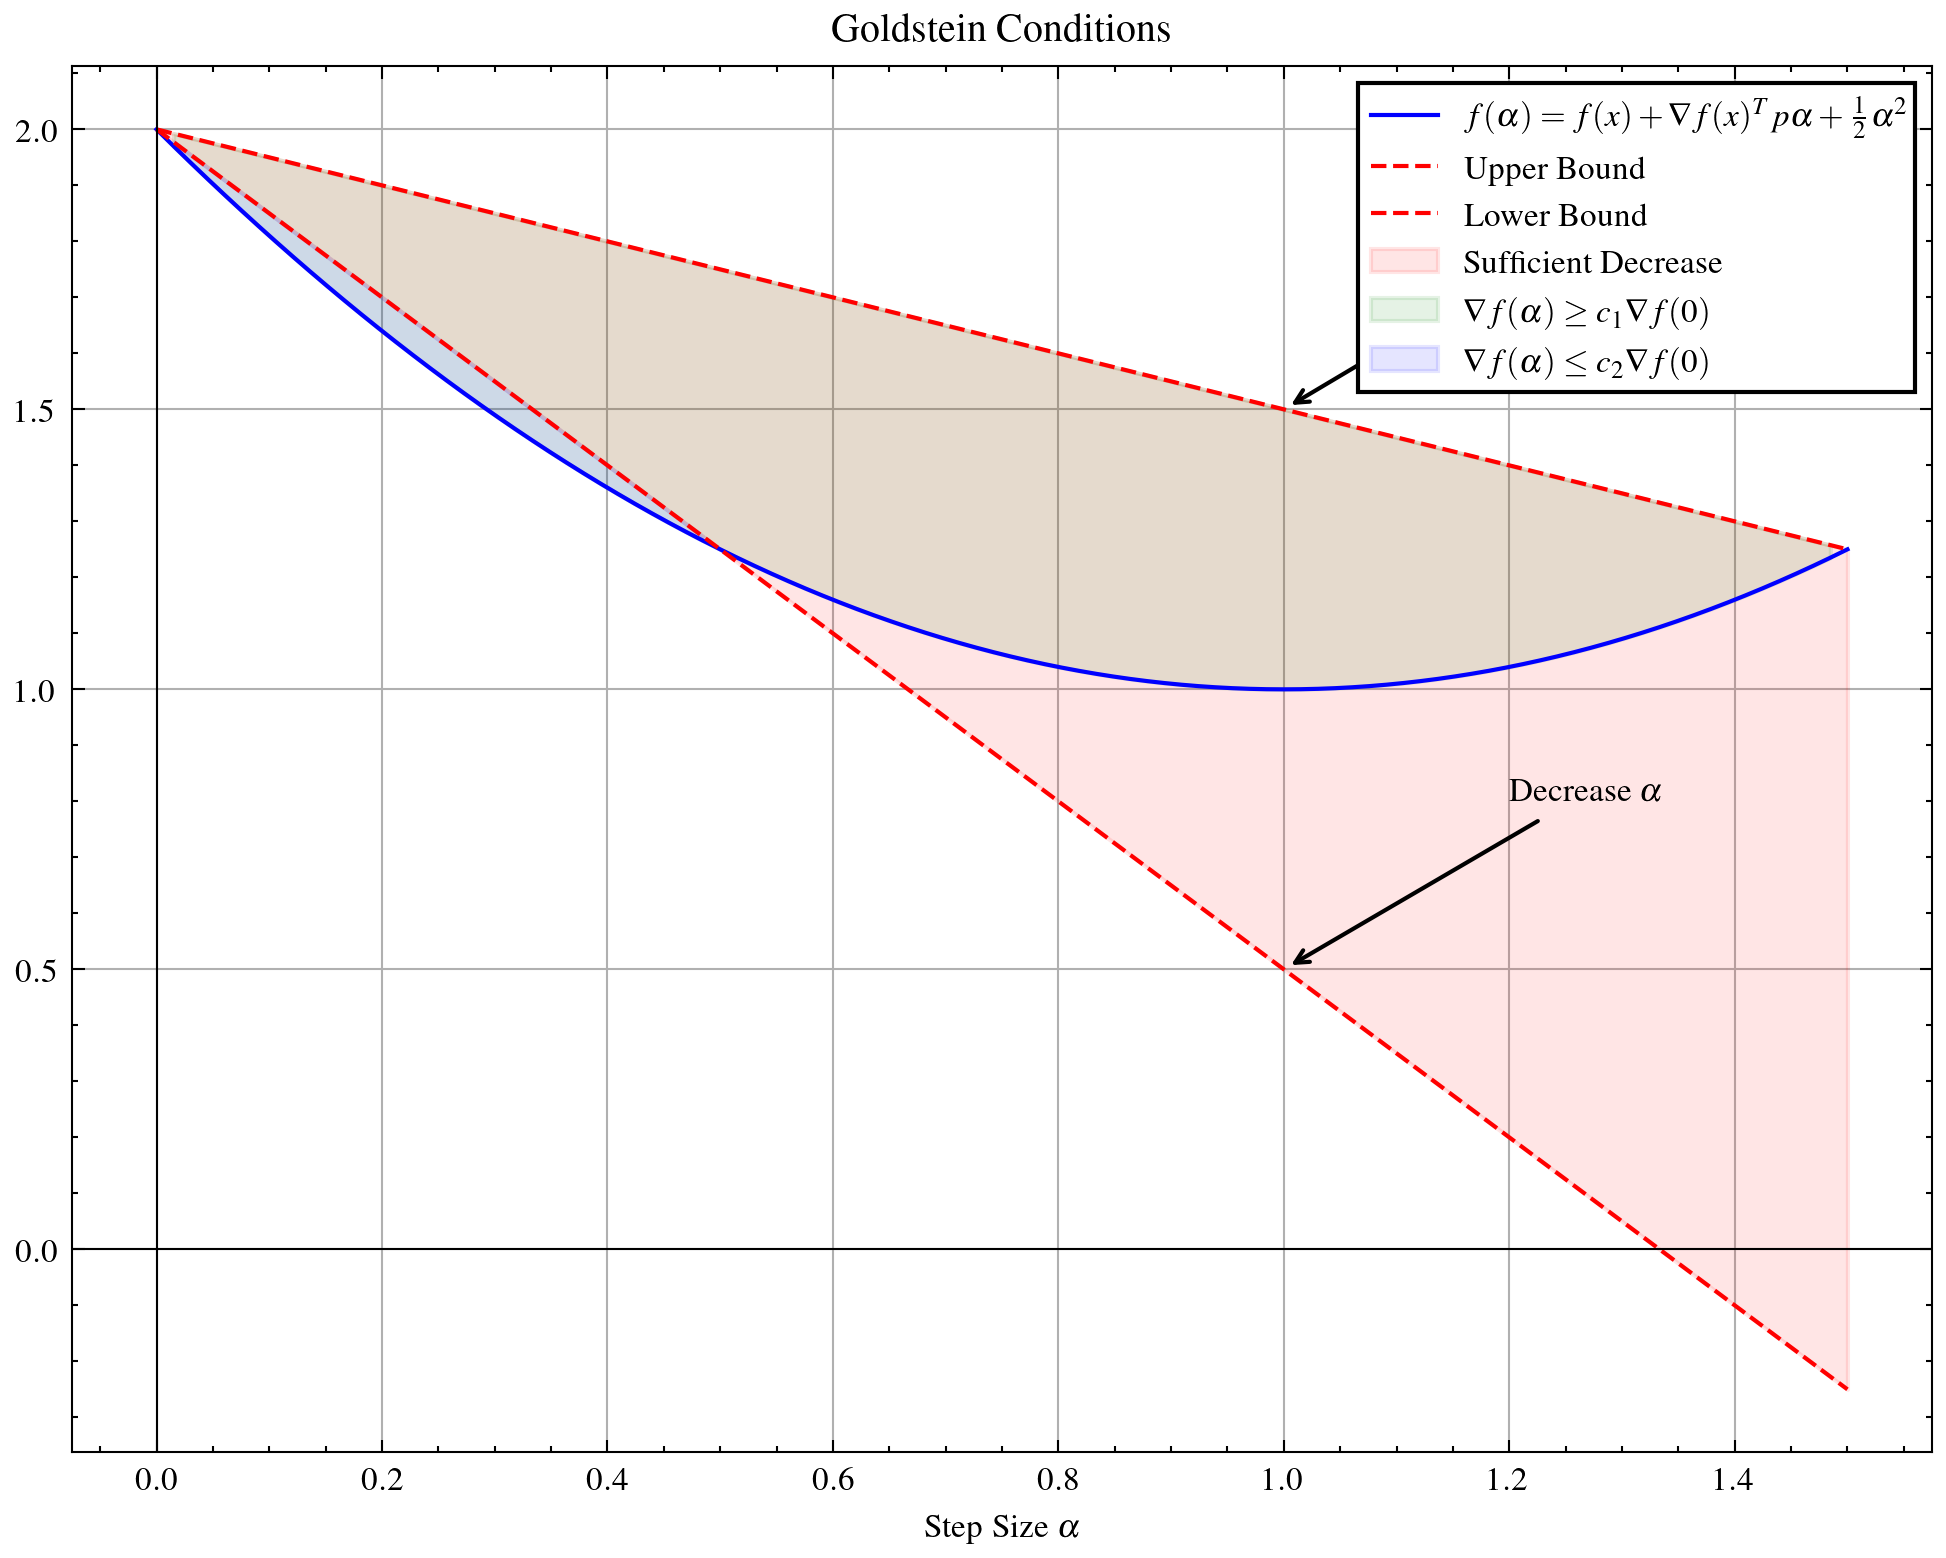
\includegraphics[scale=0.5]{figures/goldstein_conditions.png}
\begin{itemize}
    \item \textbf{Sufficient decrease:} $f(x_k + \alpha p_k) \leq f(x_k) + c_1 \alpha \ip{\nabla f(x_k), p_k}$. If this fails, decrease $\alpha$ because it is too large.
    \item \textbf{Curvature condition:} $f(x_k + \alpha p_k) \geq f(x_k) + c_2 \alpha \ip{\nabla f(x_k), p_k}$. If this fails, increase $\alpha$ because it is too small.
    \item Goldstein conditions are more robust than Armijo conditions.
\end{itemize}

\subsubsection*{Wolfe conditions}
Choose $0 < c_1 < c_2 < 1$.
\begin{itemize}
    \item \textbf{Sufficient decrease:} $f(x_k + \alpha p_k) \leq f(x_k) + c_1 \alpha \ip{\nabla f(x_k), p_k}$. If this fails, decrease $\alpha$ because it is too large.
    \item \textbf{Curvature condition:} $\ip{\nabla f(x_k + \alpha p_k)}{p_k} \geq c_2 \ip{\nabla f(x_k)}{p_k}$. If this fails, increase $\alpha$ because it is too small.
    \item Wolfe conditions are more robust than Goldstein conditions.
\end{itemize}


